\chapter{Introduzione}

\section{Le basi del machine learning}

\subsubsection{Gli ingredienti del machine learning:}

\begin{itemize}
  \item [$\Rightarrow$] \fancyglitter{Task}: specifica di cosa si vuole fare;
  \item [$\Rightarrow$] \fancyglitter{Modelli}: il modello matematico per affrontare un determinato task;
  \item [$\Rightarrow$] \fancyglitter{Features}: il modo con cui sono descritti gli esempi.
\end{itemize}

\nt{L'\fancyglitter{apprendimento automatico} ruota attorno all'idea di estrarre una regola generale per risolvere un problema a partire da problemi già risolti.}

\ex{Etichettatura delle email spam}{
  \begin{center}
    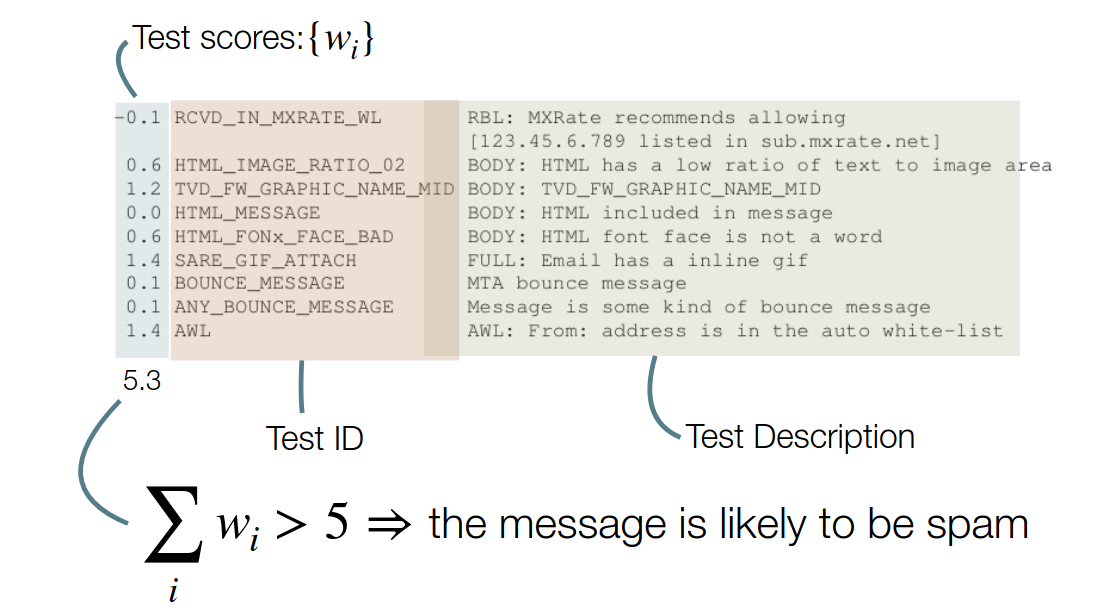
\includegraphics[scale=0.3]{01-Introduzione/Spam.png}
  \end{center}
  SpamAssassin è un filtro open-source usato per filtrare lo spam. Esso non lavora sul testo, ma su alcune \textit{feature} della mail. 
  \begin{center}
    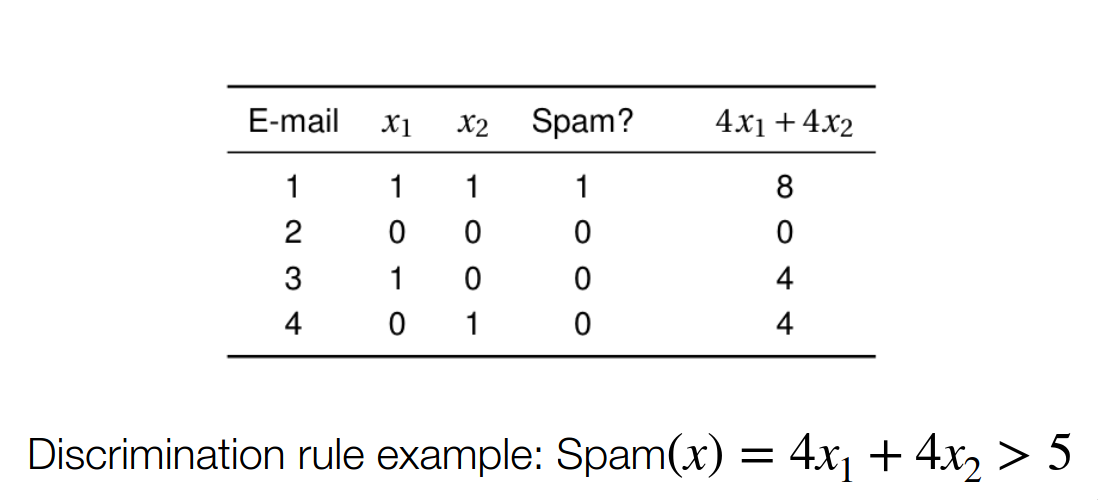
\includegraphics[scale=0.3]{01-Introduzione/Spam2.png}
  \end{center}
}

\dfn{Apprendimento automatico}{
  L'apprendimento automatico è lo studio sistematico di algoritmi e sistemi che migliorano le loro conoscenze e performance con l'esperienza.

  L'apprendimento automatico è interessato a usare le giuste features per costruire il giusto modello per ottenere buone performance sul giusto task.
}

\qs{}{
  L'apprendimento automatico come può aiutarci a risolvere un task?
}
\begin{figure}[h]
  \centering
  \begin{minipage}{0.45\textwidth}
    \centering
    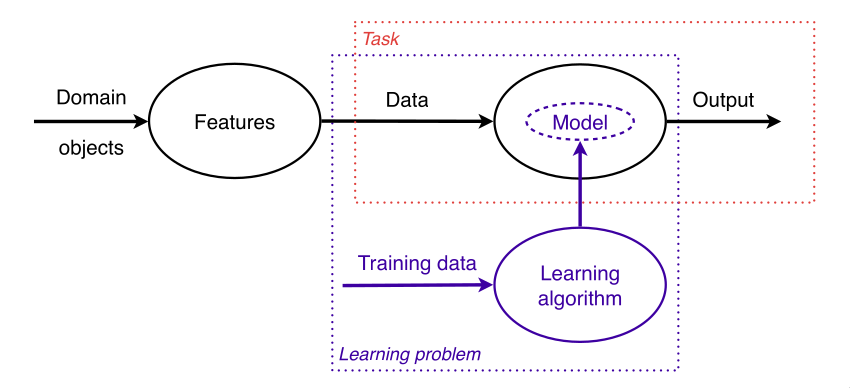
\includegraphics[scale=0.3]{01-Introduzione/ML.png}
  \end{minipage}\hfill
  \begin{minipage}{0.45\textwidth}
    \centering
    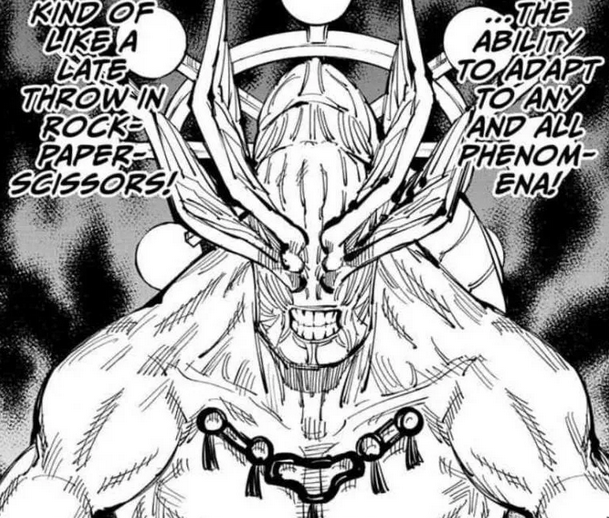
\includegraphics[scale=0.3]{01-Introduzione/Maho.png}
  \end{minipage}
\end{figure}

  \subsubsection{}
Dal dominio dell'applicazione arrivano degli oggetti descritti tramite features che vengono utilizzate per creare dei \fancyglitter{training data} e un \fancyglitter{dataset}. Questi vengono usati per costruire un modello per calcolare un output.

\nt{Per risolvere un task bisogna sfruttare un modello. Per risolvere un problema di apprendimento bisogna trovare un algoritmo di apprendimento.}

\subsection{Tasks}

\dfn{Tasks predittivi}{
  Un task predittivo è focalizzato sul prevedere una variabile sulla base degli esempi. Si parte da problemi vecchi per trovare la soluzione a \newfancyglitter{nuovi} problemi.
}

\cor{Overfitting}{
  L'Overfitting è un adattamento eccessivo al dataset di allenamento per cui, messi di fronte a nuovi problemi, non si riesce a trovare una soluzione soddisfacente.
}

\subsubsection{I tasks predittivi possono essere:}

\begin{itemize}
  \item \fancyglitter{Binari e Multi-classe:} di categorizzazione.
  \item \fancyglitter{Regressivi:} con un target numerico.
  \item \fancyglitter{Clustering:} un target sconosciuto.
\end{itemize}

\nt{IL Clustering fa anche parte dei tasks descrittivi.}

\dfn{Tasks descrittivi}{
  Un task descrittivo si concentra sul fornire regolarità nel dataset.
}


  \begin{center}
    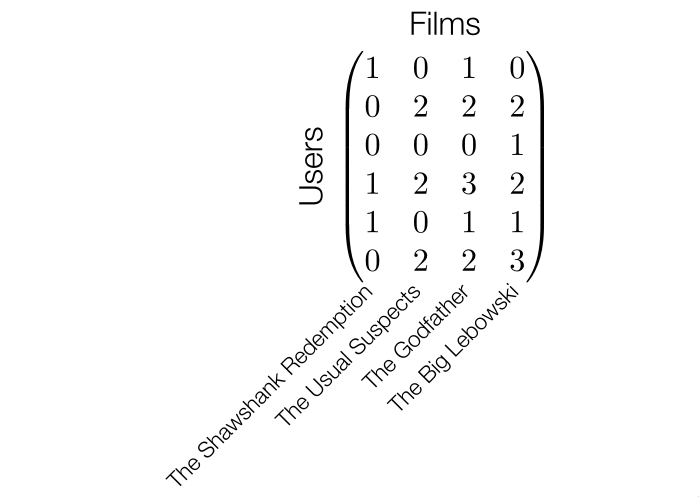
\includegraphics[scale=0.3]{01-Introduzione/M1.png}
  \end{center}

  \subsubsection{}
  Questa matrice rappresenta i voti dati da utenti a dei film. Si vogliono estrapolare le caratteristiche di questi film che hanno generato questi voti. Guardando questa matrice individualmente è difficile, per cui si compone con altre matrici.

  \begin{center} 
    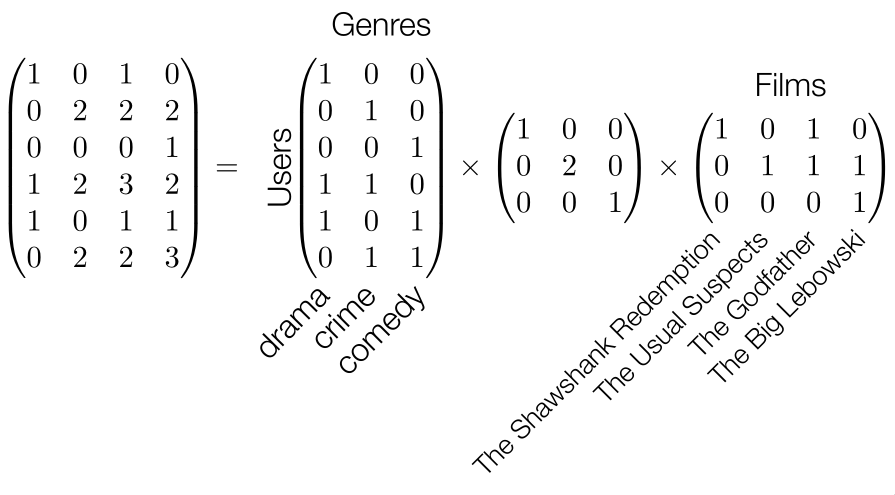
\includegraphics[scale=0.3]{01-Introduzione/M2.png}
  \end{center}

\subsection{Modelli}

\subsubsection{Ci sono 3 possibili tipi di modelli:}

\begin{itemize}
  \item \fancyglitter{Geometrici:} modelli che usano l'intuizione dalla geometria per risolvere il problema;
  \item \fancyglitter{Probabilistici:} usano il calcolo delle probabilità;
  \item \fancyglitter{Logici}.
\end{itemize}

\dfn{Modelli geometrici}{
  Nei modelli geometrici gli esempi sono punti di uno spazio vettoriale e la loro classificazione corrisponde a trovare un iperpiano che separi i punti positivi da quelli negativi.

}

\ex{Modello geometrico}{
  
  \begin{center} 
    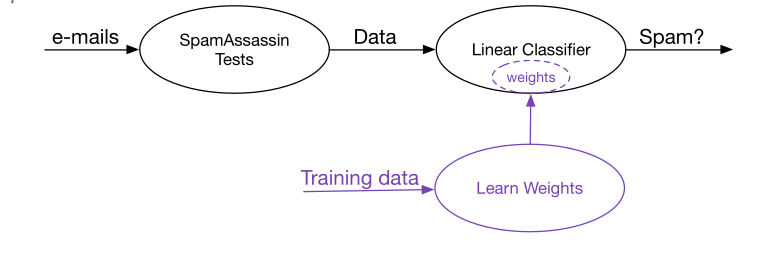
\includegraphics[scale=0.5]{01-Introduzione/Spam3.png}
  \end{center}
}

\dfn{Modelli probabilistici}{
Nei modelli probabilistici si fanno delle stime con dei classificatori probabilistici. Dopo di che si usano delle regole di decisione.

}

\ex{Modello probabilistico}{
  
  \begin{center} 
    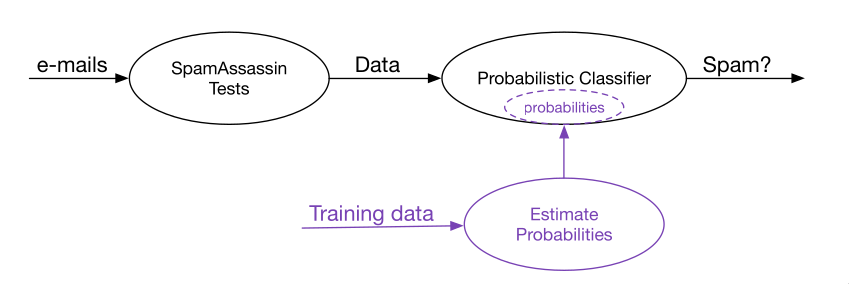
\includegraphics[scale=0.5]{01-Introduzione/Spam4.png}
  \end{center}
}

\nt{Uno degli algoritmi più semplici che si utilizza con i modelli probabilistici è l'assunzione di Naive Bayes. Si assume che x1 e x2 siano indipendenti tra loro per cui si possono calcolare solo i valori di x1 e di x2 individualmente.}



\dfn{Modelli logici}{
 Nei modelli logici si utilizza la logica. Si hanno una serie di regole.
}

\ex{Modello logico}{
  
  \begin{center} 
    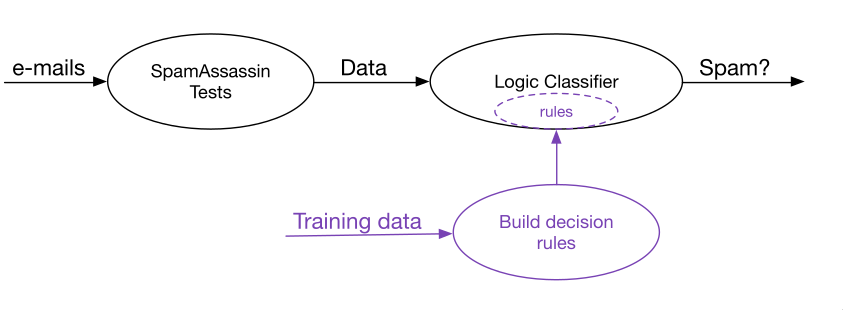
\includegraphics[scale=0.5]{01-Introduzione/Spam5.png}
  \end{center}
}

\subsection{Features}

\dfn{Features}{
  Il modo in cui si descrivono i propri dati. Possono facilitare il lavoro di apprendimento se correttamente usate.
}

\ex{Coseno}{
    
  \begin{center} 
    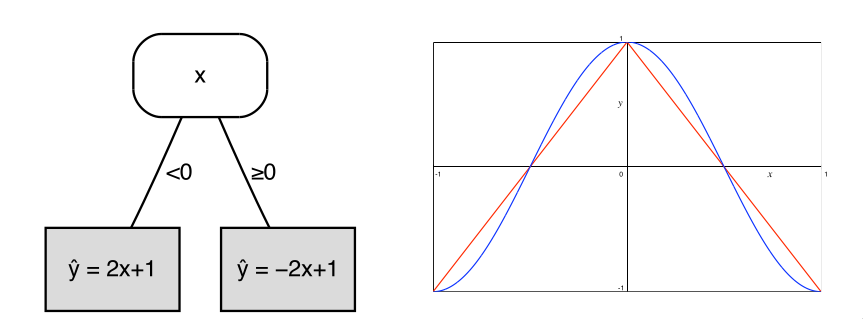
\includegraphics[scale=0.5]{01-Introduzione/COS.png}
  \end{center}

  Due rappresentazioni della funzione coseno: a destra si utilizza una variabile di regressione, a destra un'approssimazione lineare.
}

